\documentclass[12pt, parskip=full*, abstract]{scrartcl}
\usepackage{stil}

\addbibresource{bibliography.bib}

% \title{Consequences of the sun}
\title{Titan's interaction with Saturn's magnetosphere}

\author{Alexander Ek, John Persson, Björn Sundin}

\begin{document}
\maketitle
\vspace{5mm}
% \begin{abstract}
% 	In this brief non-systematic literature review we attempt to summarize the scientific knowledge about Titan's interaction with the Kronian magnetosphere.
% \end{abstract}

\newpage
\tableofcontents
\newpage

\section{Introduction}

% Cassini-Huygens was launched in 
% Pioneer 11, Voyager 2, Voyager 1, Cassini-Huygens
% Describe the different regions of the magnetosphere
% Sources and sinks of plasma
% Introduce saturn
A magnetosphere is a region around a body in space which is partially shielded from external plasma flow by its own magnetic field exerting pressure against it \parencite{encyclopedia-magnetospheres}. The magnetic field is \say{draped} around the body, and meets the oncoming flow at a \textit{magnetopause} where the pressures from the external plasma and the magnetic field are equal. On the wake side, a \textit{magnetotail} forms as the magnetic field is stretched out. Some bodies with no intrinsic magnetic field can also form a similar structure, as is the case for Venus and Saturn's biggest moon Titan (see Section \ref{s:induced-magnetosphere}). In the cases of the planets, the oncoming plasma flow is primarily the solar wind. 

Saturn has a conducting supercritical fluid hydrogen interior which through a process called magnetohydrodynamic (MHD) dynamo generates a magnetic moment about 600 times greater than Earth's. Its magnetic field rotates at approximately the same rate as Saturn itself, with some variation along its orbit around the Sun. Saturn's magnetosphere contains neutral and charged particles originating from various sources among which are the interstellar and solar winds, Saturn's inner icy moons (via sputtering and the geyser on Enceladus), Titan's and Saturn's atmospheres and ionospheres, and Saturn's rings \parencite{solar-system-magnetospheres}. Due to friction in Saturn's atmosphere and ionosphere, the magnetospheric plasma rotates with the same period as Saturn spins about its axis. It is mostly concentrated around the equator because of the centrifugal forces in Saturn's rotating reference frame.

% was discovered in 1655 by Christiaan Huygens,
Titan is Saturn's largest moon and the second largest moon in our solar system \parencite{fundamental-planetary-science}. It is an icy moon with a radius of \SI{2575}{\kilo\metre}, a density of \SI{1880}{\kilogram\per\metre^3}, and a surface pressure of \SI{1.44}{\bar}. Unlike all other moons in our solar system, Titan has an atmosphere with a higher surface pressure than Earth's. The atmosphere consists mainly of nitrogen and a smaller amount of methane. With an inclination of about \SI{0.4}{\degree}, the moon orbits close to Saturn's equatorial plane. Titan has no intrinsic magnetic field but having an orbit at 20 Saturn radii places it near the boundary of the varying Saturnian magnetic field on the Sun-facing side. This combination of a dense atmosphere and the lack of an intrinsic magnetic field makes its interaction with the surrounding plasma unlike that of any other moon in the solar system. 

Four spacecraft have visited Saturn so far; Pioneer 11 (launched 1973, flyby 1979), Voyagers 1 and 2 (launched 1977, flybys 1980 and 1981 respectively), and Cassini-Huygens (launched 1997, flyby 2004) \parencite{encyclopedia-missions}. A major objective of the Voyager 1 project was to study Titan and its interactions with the surrounding magnetosphere \parencite{hartle-1982}. The Cassini spacecraft which was in orbit around Saturn until it ended its mission by crashing into Saturn's atmosphere in 2017 \parencite{cassini-2019} has provided much more detailed observations of the dynamics of the Kronian magnetosphere than those from the Pioneer 10 and Voyager 1 and 2 spacecraft which only briefly passed through it \parencite{encyclopedia-magnetospheres}. 


\section{Interactions between Titan and Saturn's magnetosphere}

\subsection{Titan's induced magnetosphere}\label{s:induced-magnetosphere}
There are two flows of charged particles across Titan; one is from the solar wind and one is from Saturn's magnetospheric plasma \parencite{ionosphere-magnetosphere-interaction-coates}. The latter corotates with Saturn's rotation period of approximately $\tau_\text{plasma}=\SI{10.5}{\hour}$, while Titan's rotation period around Saturn is $\tau_\text{titan}=\SI{15.9}{\day}$ \parencite{fundamental-planetary-science}. Neglecting the eccentricity of Titan ($e\approx0.03$) and noting that Titan orbits with a semimajor axis of $a=\SI{1222}{\mega\metre}$, this implies that the magnetospheric plasma flows at a speed of approximately
\begin{equation}
	2\pi a\left(\frac{1}{\tau_\text{plasma}} - \frac{1}{\tau_\text{titan}}\right)\approx\SI{198}{\kilo\metre\per\second}
\end{equation}
relative to Titan. For comparison, the solar wind at Earth's orbit is normally around \SI{440}{\kilo\metre\per\second}, although it can vary greatly \parencite{encyclopedia-solar-wind}. Since Titan orbits in the same direction as saturn spins around its axis, the ram side of this plasma flux is \say{behind} Titan rather than in front. The difference in direction between the flow of particles from the Sun and from the magnetospheric plasma changes during the local day on Titan, as illustrated in Figure \ref{fig:wakes}. When Titan is inside Saturn's magnetosphere it is partially shielded from the solar wind, meaning that the corotating plasma is the dominating flow \parencite{ionosphere-magnetosphere-interaction-coates}. This is the situation that has been most studied since most observations by spacecraft have been in such conditions.

\begin{figure}[htbp]
	\centering
	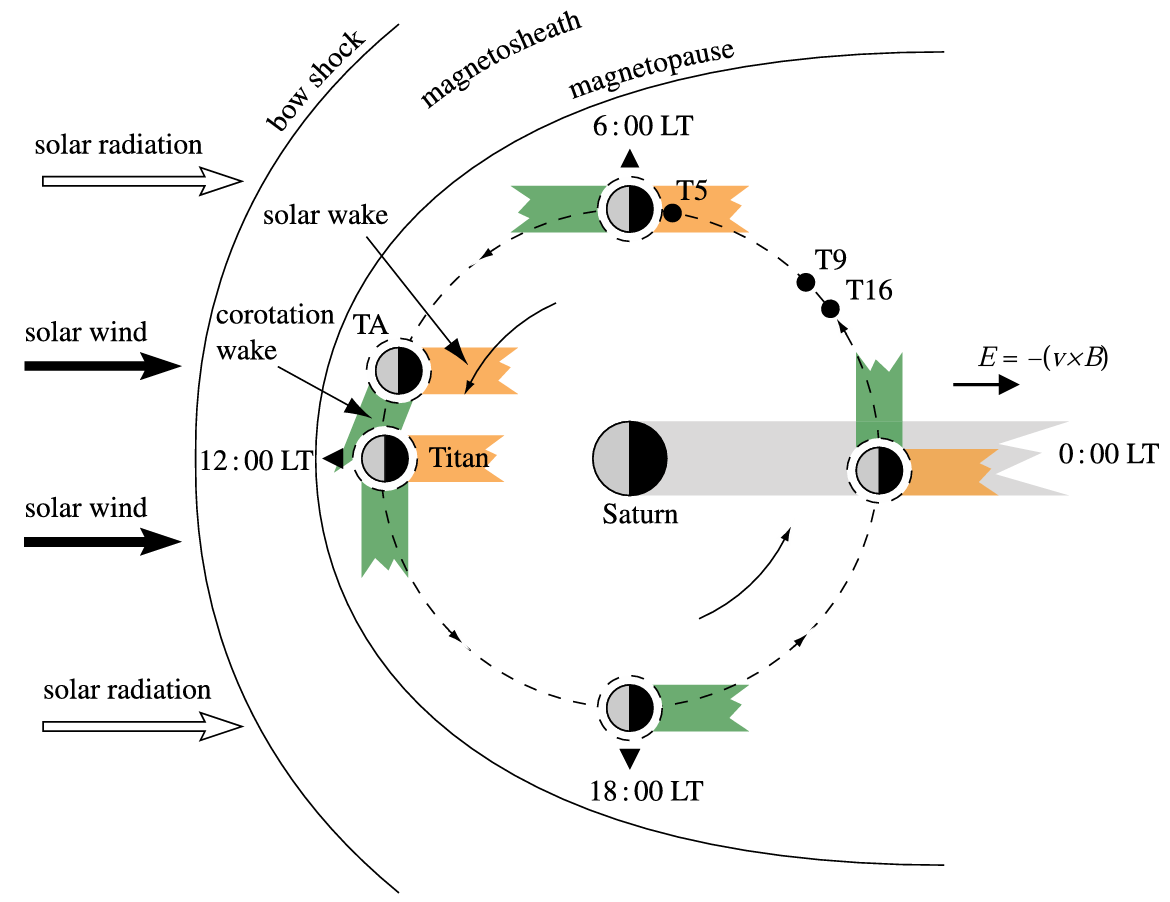
\includegraphics[width=0.7\textwidth]{wakes}
	\caption{An illustration of Titan's two plasma flow wakes in its orbit around Saturn. Taken from \textcite{ionosphere-magnetosphere-interaction-coates}.}
	\label{fig:wakes}
\end{figure}

The magnetospheres of most planets as well as Jupiter's moon Ganymede arise from an intrinsic magnetic field generated via MHD dynamo \parencite{encyclopedia-magnetospheres}. Titan has no such magnetic field, but it possesses a conducting ionosphere. When the corotating plasma flows across Titan, currents are induced in its ionosphere that create forces that oppose the oncoming flow. This results in an induced magnetosphere around the body, with a magnetotail \say{in front}. The magnetic field around Titan changes rapidly only very close to its surface. In contrast to the planetary magnetospheres which are subjected to the supersonic solar wind, the induced magnetosphere of Titan has no bow shock since the oncoming plasma flow is slower than both the Alfvén speed and the sound speed of the plasma. 

% \parencite{encyclopedia-magnetospheres}:
%A magnetosphere is a region around a body in space which is partially shielded from external plasma flow by its own magnetic field exerting magnetic pressure against the flow. However, even bodies with no intrinsic magnetic field can form cavities in the plasma flow which have properties that are similar to true magnetospheres. The magnetopause is the surface defining the boundary of the magnetosphere. The term magnetosphere was originally defined as a region above the Earth's ionosphere, but the term has since expanded to include similar phenomena around other bodies in space, including moons. 

% Some bodies in the solar systems lack a substantial intrinsic magnetic field. Among these are Mars, Venus, and all moons except the Jovian moon Ganymede. If the body has a conductive interior or an ionosphere, then currents are induced that create forces that oppose the incoming external plasma flow (solar wind or magnetospheric plasma). This results in an induced magnetosphere around the body.

%A planet or moon that has an ionosphere will form an induced magnetosphere if charged particles are flowing past it \parencite{fundamental-planetary-science}. This induced magnetosphere shields the body from the external magnetic field. Titan in Saturn's magnetosphere is an example of this.
% In several analyses of data recorded by instruments on the Voyager 1 when it flew by Titan in 1980 .
% Since Titan mostly resides within Saturn's magnetosphere


Voyager 1 carried a plasma science instrument which was used to make around 20 measurements of energy spectra for electrons and ions in the wake of Titan during a flyby in 1980. In a paper by \textcite{hartle-1982}, the data from these measurements were analyzed and interpreted to give insights into the structure of Titan's magnetotail. Figure \ref{fig:1980-flyby} illustrates the trajectory of the spacecraft during the flyby, projected onto Titan's orbital plane with the X-axis pointing in the corotation direction and and Y-axis pointing towards Saturn. The flyby took place at 13:30 local solar time (as defined in Figure \ref{fig:wakes}) \parencite{ness-1982}. 

Some results from the electron measurements are presented in figures \ref{fig:wake-spectra} and \ref{fig:wake-temp-density}. The first figure shows the velocity distributions across the wake of Titan, and a clear \say{bite-out} can be seen where there are almost no electrons with speeds higher than about \SI{16}{\mega\metre\per\second} (\SI{730}{\electronvolt}). The second figure also shows that this wake region is more dense than the surroundings. This population of cold and dense electrons might be produced by ionization of exospheric particles and energy transfer via collisions with neutral atoms in Titan's atmosphere. Comparison of the observed ion speed distributions with synthetic ones indicated the pickup of \ce{H+} from Titan's exosphere by the corotating flow on the sun-facing side outside the tail, as well as a retarded plasma flow close to the boundary of the magnetotail. The latter is thought to be due to \textit{mass loading} of the magnetic field lines by \ce{N+} and \ce{N2+}/\ce{H2CN+}.

\begin{figure}[htbp]
	\centering
	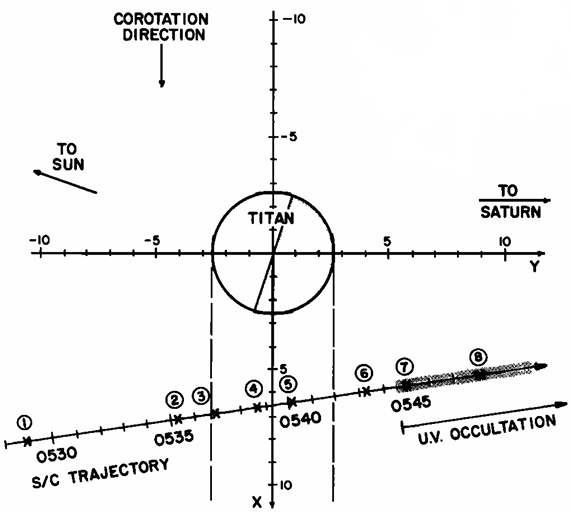
\includegraphics[width=0.7\textwidth]{1980-flyby}
	\caption{An illustration of the flyby of Titan by Voyager 1 on the 12th of November 1980. The trajectory is projected onto Titan's orbital plane. The units of the coordinates are \si{\mega\metre} and the numbers along the trajectory are the spacecraft-local time points. Adapted from \textcite{hartle-1982}.}
	\label{fig:1980-flyby}
\end{figure}


\begin{figure}[htbp]
	\begin{subfigure}{\textwidth}
		\centering
		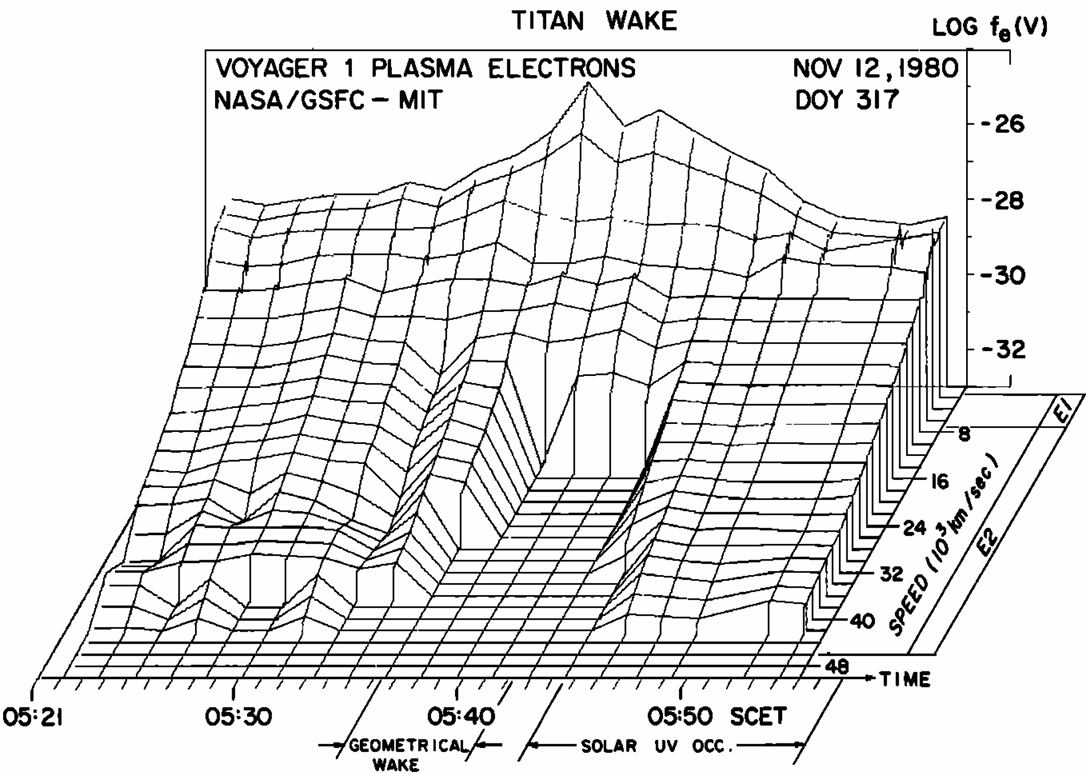
\includegraphics[width=0.8\textwidth]{wake-spectra}
		\caption{Electron speed spectra.}
		\label{fig:wake-spectra}	
	\end{subfigure}
	\begin{subfigure}{\textwidth}
		\centering
		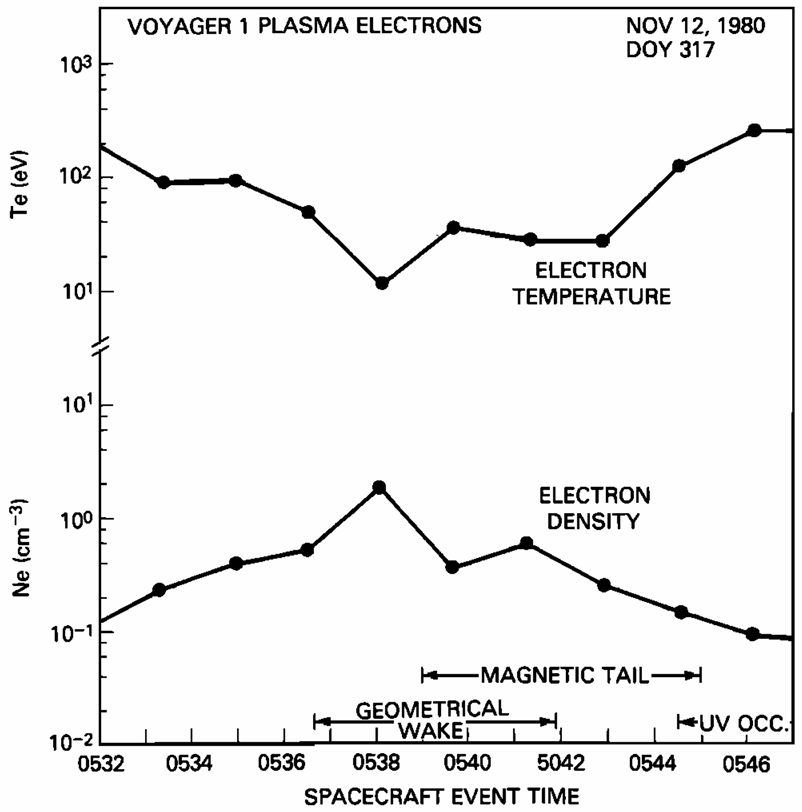
\includegraphics[width=0.7\textwidth]{wake-temp-density}
		\caption{Electron temperature and density measurements.}
		\label{fig:wake-temp-density}
	\end{subfigure}
	\caption{Plots from \textcite{hartle-1982} of electron energy spectra, temperatures, and number densities in Titan's wake recorded by the plasma science experiment on Voyager 1.}
\end{figure}

The Voyager 1 spacecraft also had a magnetometer which recorded measurements of the magnetic field along its trajectory during the same flyby. These were analyzed by \textcite{ness-1982}. The magnetotail was found to be perturbed by about \SI{20}{\degree} from the coration direction towards Saturn, likely caused by the difference in irradiation from the Sun between the night and day sides of Titan's ionosphere. Figure \ref{fig:wake-field} illustrates possible magnetic field lines based on this data.

\begin{figure}[htbp]
	\centering
	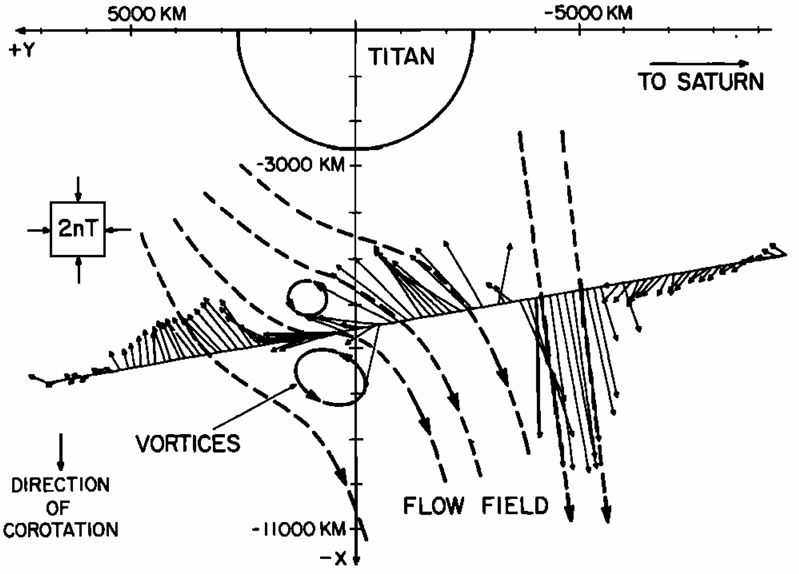
\includegraphics[width=0.7\textwidth]{wake-field}
	\caption{Magnetic field lines in the wake of Titan as inferred by \textcite{ness-1982} based on magnetometer data from Voyager 1.}
	\label{fig:wake-field}
\end{figure}

During Cassini's T9 flyby, the magnetotail was analyzed at mid-ranges, 5-6 Titan radii downstream in terms of magnetometer data and electron energy and count by \textcite{Magnetotail-T9}. This paper corroborates the structure of Titan's magnetotail, showing two lobes with a current sheet in-between. This paper also finds that the measured magnetic field of the ingoing lobe, if extrapolated intersects the ionosphere of Titan. Additionally, a high plasma density is detected in this region, suggesting that this plasma is escaping Titan along the magnetic field lines. Large asymmetries are also found
between the two tails, which are thought to be due to the connection of the lobes to the dayside for the inbound and the nightside for the outbound.

In a paper by \textcite{alfven-wing-structure}, the data from the T122-T126 Cassini flybys of Titan were used to analyze its magnetotail structure. The magnetotail was found to display variations over time and space. In two of the flybys (T123 and T124) an Alfvén wing-like structure was observed in the magnetic field around Titan. Alfvénic wing-like structures are created when Titan is exposed to sub-magnetosonic flow from Saturn's magnetospheric plasma and is a direct consequence of Titan not having an internal magnetosphere. The wing-like structures connect the field lines of Saturn's magnetosphere with Titan's ionosphere. A bipoloar magnetotail with an embedded neutral current sheet in the magnetotail was also observed in the T122 flyby, as has been observed earlier by the Voyager 1 flybys \parencite{ness-1982}.

% \begin{figure}[htbp]
% 	\centering
% 	\includegraphics[width=0.7\textwidth]{alvenicwings}
% 	\caption{}
% 	\label{fig:alvenicwings}
% \end{figure}

\subsection{Titan's plasma environment}
A 2009 study by \textcite{Rymer-class} classifies Titan's background plasma environment into four different categories based on electron thermal data from 54 encounters on Titan by Cassini as follows. The categories refer to regions of Saturn's magnetosphere, not regions of Titan's induced magnetosphere. 

\begin{enumerate}
	\item The \textbf{plasma sheet} contains high energy electrons whose peak enegy is on the order of $100$s \si{\electronvolt}. The electron density is also high in this region with fluxes at \SI{e6}{\centi\metre^{-2}\second^{-1}\steradian^{-1}}. This was the most common environment, with 19 encounters.
	\item The \textbf{lobe-like} region also has high energy electrons, with peak energies similar to or higher than that of the plasma sheet. The electron density is however smaller, with fluxes an order of magnitude less. Eight encounters with this environment were made.
	\item The \textbf{magnetosheath} is encountered outside of the magnetopause, and thus consists of plasma from the solar wind. In this region electrons are of lower energy, but higher density than the previous two classes. Two encounters with this environment were made.
	\item The \textbf{bi-modal} region is highly variable, containg two seperate electron populations. One is similar in energy to the plasma sheet or lobe-like category. The other population is less energetic but more dense and consists of a so called local pick-up population that comes from a neutral cloud, where produced electrons are quickly picked up by the co-rotation with Saturn gaining energy on the order of tenths of \si{\electronvolt}. The electron energy seen is higher though, which is thought to be explained by these electrons originating from photoionization of larger ions where the energy released is on the order of \SI{10}{\electronvolt}. These heavy ions are believed to be water groups which originate in the inner magnetosphere of Saturn from the moon Enceladus and migrate outwards to Titan. Five encounters of this environment were made.

\end{enumerate}

A paper by \textcite{Smith-WithOrWithoutTitan} further examines more encounters by Cassini, establishing that 45\% of encounters were plasma sheet, 38\% were lobe-like, and 6\% magnetosheath. The plasma environment along Titan's obit when the moon is not currently present was also examined. Here 55\% of encounters were plasma sheet, 24\% were lobe-like, and 12\% were magnetosheath. This suggests that the presence of Titan lowers the probablity of experiencing the magnetosheath, meaning that Titan extends the magnetopause of Saturn outwards. The authors could not conclude this however, due to possible sampling bias that needs to be analyzed more rigorously. 

An earlier paper by \textcite{Wei-WithOrWithoutTitan} draws a similar conclusion. This study looks at the specific time interval of 09:00 - 15:00 Saturn local time (SLT) and examines the plasma environment in 26 cases with and 37 without Titan present. The percentage of time in the magnetosheath was 3.37\% near Titan and 10.37\% away from Titan, which is statistically significant. The implication of this is that the compression of the plasma is hindered by Titan's presence. \textcite{Smith-WithOrWithoutTitan} also finds that the bi-modal environment is more prevalant in the vicinity of Titan compared to the orbit of Titan without the moon present. This suggests that ionization is greater with Titan present, as the origin of the low energy population of the bi-modal environment is thought to be pick-up ions. 

An additional classification of the plasma environment dubbed \textbf{dense plasma region} is also recognized by \textcite{Smith-WithOrWithoutTitan}. In this environment the electron energies can be compared to the low energy plasma of the bi-modal environment, but the higher energy electrons seen in the bi-modal environment are not present. Additionally, the environment is more long-lived than the bi-modal low energy electrons. This environment was seen during dusk, and no theory of its origin could be found.%Maybe unneccessary //John

\subsection{Energetic particle interactions}

% Titan is a weaker plasma source than the inner moon Enceladus which emits large amounts of vapor that is quickly ionized, forming a torus of plasma around Saturn. 

% I thought that this was slightly inaccurate: the whole reason for the design of the MIMI was to make images of ENAs because it was known that they are produced in charge-exchange collisions - the instrument didn't discover this mechanism, it only imaged ENA distributions. I adapted the paragraph and added some relevant explanation which I had in my notes //Björn

%These interactions were captured using the magnetosphere imaging instrument (MIMI) and the ion and neutral mass spectrometer (INMS) onboard the Cassini spacecraft. The instruments were able to detect that energetic ions from Saturn's magnetosphere undergo charge-exchange collisions with slow neutral atoms in Titan's upper atmosphere, producing energetic neutral atoms (ENAs). The reaction describing a charge-exchange collision is \ce{X+ + Y -> X_{ENA} + Y+}, where \ce{X+} is the energetic ion, \ce{Y} is the colliding cold neutral atom, \ce{X_{ENA}} is the resulting energetic neutral atom, and \ce{Y+} is the ionized particle. Charge-exchange collisions is one of the reasons for Titan's exosphere deviating from thermal equilibrium, with some other reasons being sputtering and photodissociation. Data from Cassini flybys indicated that the highest amount of particle collisions occured in the lower atmosphere causing most of the produced ENAs to be absorbed, resulting in a darker region in the ENA image of Titan's exosphere as can be seen in figure \ref{fig:ENA-image}.

The fact that Titan lacks an intrinsic magnetic field makes its atmosphere directly susceptible to the oncoming plasma flow. \textcite{titan-exosphere-interaction} analyzed some observations from the Cassini spacecraft relating to energetic particle interactions in Titan's exosphere. Energetic neutral atoms (ENAs) result from charge-exchange collisions where a slow neutral atom in Titan's atmosphere transfers an electron to an energetic +1 charge ion from the oncoming flow \parencite{titan-exosphere-interaction}. These ENAs were imaged by the magnetosphere imaging instrument (MIMI) on the Cassini spacecraft from afar, while the ion and neutral mass spectrometer instrument (INMS) performed measurements directly inside Titan's exosphere. ENAs were imaged as a proxy for energetic charged particles because neutral particles are not affected by electromagnetic fields and follow paths similar to those that photons would take. 

From the in-situ measurements by the INMS it was deduced that Titan's exobase is located at about 1425 km altitude and that it has a temperature of 149 K. Figure \ref{fig:ENA-image} shows an ENA image captured by the MIMI. Below an altitude of about 1 Mm above Titan's surface in its lower atmosphere, the collision frequency of particles is so high that most of the produced ENAs are absorbed, which results in a darker region in the ENA image of Titan's exosphere. The energy of the incoming energetic protons and oxygen ions from Saturn's magnetosphere is therefore deposited mostly in the dense lower atmosphere. The exosphere was also found to deviate from thermal equilibrium, partly due to the input of energetic ions from Saturn's magnetosphere.

%The reaction describing a charge-exchange collision is \ce{X+ + Y -> X_{ENA} + Y+}, where \ce{X+} is the energetic ion, \ce{Y} is the colliding cold neutral atom, \ce{X_{ENA}} is the resulting energetic neutral atom, and \ce{Y+} is the ionized particle.

\begin{figure}[htbp]
	\centering
	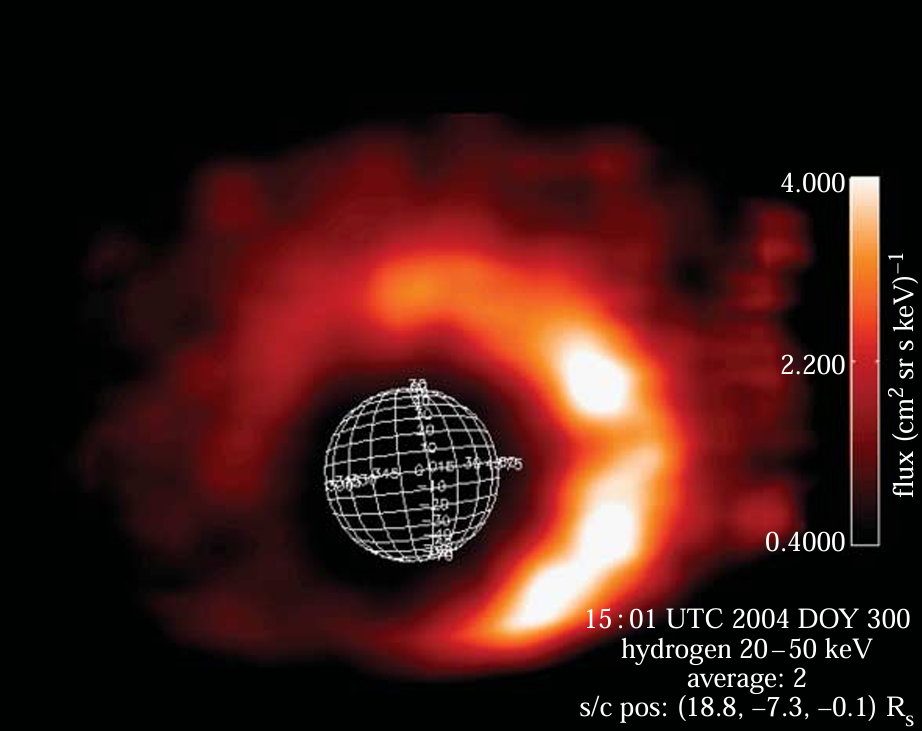
\includegraphics[width=0.7\textwidth]{ENA-image}
	\caption{Image of ENAs in Titan's exosphere taken by the MIMI during a Cassini flyby. Taken from \textcite{titan-exosphere-interaction}.}
	\label{fig:ENA-image}
\end{figure}

%All magnetospheres in the solar system contain populations of highly energetic particles which deviate from the thermal equilibrium Maxwell-Boltzmann distribution function \parencite{encyclopedia-magnetospheres}. The observed fluxes of such particles are too high to be solely accounted for by the solar wind. In the cases of the gas giants, some particles are accelerated to high energies by planetary rotation. These high-energy particles also create strong currents around the equator which in turn modify the magnetic field. The significant populations of energetic particles in the gas giants' magnetospheres result in an expanded magnetopause due to the increased pressure. Energetic particles at the gas giants can be lost via absorption by their rings and satellites.

%Cassini was equipped with an instrument that took pictures of particle fluxes in the magnetosphere (one of the three sensors of the magnetosphere imaging instrument (MIMI)) \parencite{titan-exosphere-interaction}. This detector can be likened to a telescope which collects neutral particles instead of photons. High-energy neutrals result from collisions with energetic ions (charge-exchange collisions) and therefore the observations provide information about the magnetospheric plasma.


% Source of plasma
 
% \subsection{}

\section{Conclusions}
In this brief literature review we attempted to summarize the scientific knowledge about Titan's interaction with the Kronian magnetosphere. The articles were chosen rather arbitrarily, and for this reason as well as length constraints the review is incomplete. 

Titan is a unique moon with its thick nitrogen-methane atmosphere. During its orbit it experiences various plasma environments both within and outside Saturn's magnetosphere. While within it, Titan is exposed to an energetic plasma that corotates with Saturn at a speed of about \SI{200}{\kilo\metre\per\second} relative to Titan. Energetic ions in Saturn's magnetosphere interact with Titan's atmosphere which gives rise to phenomena such as charge-exchange collisions, and perturbs the moon's exospheric plasma from thermal equilibrium. 

Currents in Titan's ionosphere induced by the corotating plasma create a magnetosphere-like cavity around the moon comparable to that around Venus (which has in common with Titan that it lacks an intrinsic magnetic field), complete with a magnetotail in front. A difference between Titan's and Venus' induced magnetospheres is that Titan's magnetotail is perturbed in different directions depending on the solar local time, while in the case of Venus the plasma flow direction always coincides with the direction of the sun. 


\newpage
\printbibliography

\end{document}


